\begin{frame}{\small Global localisation: Το δεύτερο μεγαλύτερο πρόβλημα ρομποτικής κινητής βάσης}

  \vspace{-1cm}
  \noindent\makebox[0.6\linewidth][c]{%o
  \begin{minipage}{0.6\linewidth}

    \begin{figure}
      \input{./figures/slides/ch5/localisation_problems_pie.tex}
      \vspace{-1.5cm}
      \caption{\scriptsize Ποσοστά έρευνας στα προβλήματα εκτίμησης στάσης. Πηγή:
               Prabin Kumar Panigrahi and Sukant Kishoro Bisoy.  ``Localization
               strategies for autonomous mobile robots: A review",
               \textit{Journal of King Saud University - Computer and
               Information Sciences}, Mar. 2021.}
    \end{figure}

  \end{minipage}
  }
  \hfill
  \noindent\makebox[0.3\linewidth][c]{%
  \begin{minipage}{0.3\linewidth}
    \begin{figure}
      


\tikzset{every picture/.style={line width=0.75pt}} %set default line width to 0.75pt

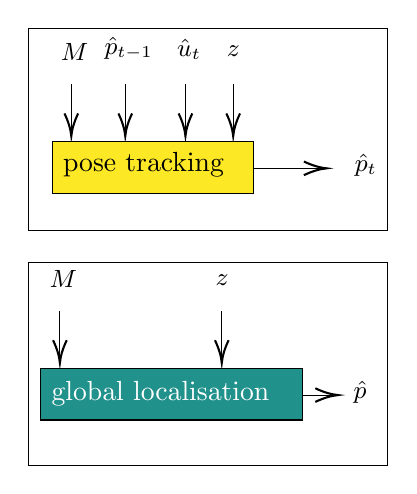
\begin{tikzpicture}[x=0.75pt,y=0.75pt,yscale=-1,xscale=1]
%uncomment if require: \path (0,300); %set diagram left start at 0, and has height of 300


%Straight Lines [id:da37620075399637964]
\draw    (130.25,28.5) -- (130.25,51.5) ;
\draw [shift={(130.25,53.5)}, rotate = 270] [color={rgb, 255:red, 0; green, 0; blue, 0 }  ][line width=0.75]    (10.93,-3.29) .. controls (6.95,-1.4) and (3.31,-0.3) .. (0,0) .. controls (3.31,0.3) and (6.95,1.4) .. (10.93,3.29)   ;
%Straight Lines [id:da8910828803681619]
\draw    (156.25,28.5) -- (156.25,51.5) ;
\draw [shift={(156.25,53.5)}, rotate = 270] [color={rgb, 255:red, 0; green, 0; blue, 0 }  ][line width=0.75]    (10.93,-3.29) .. controls (6.95,-1.4) and (3.31,-0.3) .. (0,0) .. controls (3.31,0.3) and (6.95,1.4) .. (10.93,3.29)   ;
%Straight Lines [id:da7026914270045463]
\draw    (185.25,28.5) -- (185.25,51.5) ;
\draw [shift={(185.25,53.5)}, rotate = 270] [color={rgb, 255:red, 0; green, 0; blue, 0 }  ][line width=0.75]    (10.93,-3.29) .. controls (6.95,-1.4) and (3.31,-0.3) .. (0,0) .. controls (3.31,0.3) and (6.95,1.4) .. (10.93,3.29)   ;
%Straight Lines [id:da07058947705205698]
\draw    (208.25,28.5) -- (208.25,51.5) ;
\draw [shift={(208.25,53.5)}, rotate = 270] [color={rgb, 255:red, 0; green, 0; blue, 0 }  ][line width=0.75]    (10.93,-3.29) .. controls (6.95,-1.4) and (3.31,-0.3) .. (0,0) .. controls (3.31,0.3) and (6.95,1.4) .. (10.93,3.29)   ;
%Straight Lines [id:da658480361580742]
\draw    (217.75,69) -- (251.25,69) ;
\draw [shift={(253.25,69)}, rotate = 180] [color={rgb, 255:red, 0; green, 0; blue, 0 }  ][line width=0.75]    (10.93,-3.29) .. controls (6.95,-1.4) and (3.31,-0.3) .. (0,0) .. controls (3.31,0.3) and (6.95,1.4) .. (10.93,3.29)   ;
%Straight Lines [id:da014317254825124026]
\draw    (124.75,137.75) -- (124.75,160.75) ;
\draw [shift={(124.75,162.75)}, rotate = 270] [color={rgb, 255:red, 0; green, 0; blue, 0 }  ][line width=0.75]    (10.93,-3.29) .. controls (6.95,-1.4) and (3.31,-0.3) .. (0,0) .. controls (3.31,0.3) and (6.95,1.4) .. (10.93,3.29)   ;
%Straight Lines [id:da6026375160663937]
\draw    (202.75,137.75) -- (202.75,160.75) ;
\draw [shift={(202.75,162.75)}, rotate = 270] [color={rgb, 255:red, 0; green, 0; blue, 0 }  ][line width=0.75]    (10.93,-3.29) .. controls (6.95,-1.4) and (3.31,-0.3) .. (0,0) .. controls (3.31,0.3) and (6.95,1.4) .. (10.93,3.29)   ;
%Straight Lines [id:da2508525371297663]
\draw    (241.25,178.25) -- (256.75,178.25) ;
\draw [shift={(258.75,178.25)}, rotate = 180] [color={rgb, 255:red, 0; green, 0; blue, 0 }  ][line width=0.75]    (10.93,-3.29) .. controls (6.95,-1.4) and (3.31,-0.3) .. (0,0) .. controls (3.31,0.3) and (6.95,1.4) .. (10.93,3.29)   ;
%Shape: Rectangle [id:dp5753636561604081]
\draw   (109.5,1.5) -- (282.75,1.5) -- (282.75,99) -- (109.5,99) -- cycle ;
%Shape: Rectangle [id:dp27272606446856584]
\draw   (109.5,114.5) -- (282.75,114.5) -- (282.75,212) -- (109.5,212) -- cycle ;

% Text Node
\draw  [fill={rgb, 255:red, 253; green, 232; blue, 38 }  ,fill opacity=1 ]  (121,56) -- (218,56) -- (218,81) -- (121,81) -- cycle  ;
\draw (125,60) node [anchor=north west][inner sep=0.75pt]   [align=left] {pose tracking};
% Text Node
\draw (124,7.75) node [anchor=north west][inner sep=0.75pt]   [align=left] {\small $\bm{M}$};
% Text Node
\draw (145,4.75) node [anchor=north west][inner sep=0.75pt]   [align=left] {\small $\hat{\bm{p}}_{t-1}$};
% Text Node
\draw (180,5.75) node [anchor=north west][inner sep=0.75pt]   [align=left] {\small $\hat{\bm{u}}_t$};
% Text Node
\draw (204,8.75) node [anchor=north west][inner sep=0.75pt]   [align=left] {\small $\bm{z}$};
% Text Node
\draw (265.6,61) node [anchor=north west][inner sep=0.75pt]   [align=left] {\small $\hat{\bm{p}}_{t}$};
% Text Node
\draw  [fill={rgb, 255:red, 33; green, 145; blue, 140 }  ,fill opacity=1 ]  (115.5,165.25) -- (241.5,165.25) -- (241.5,190.25) -- (115.5,190.25) -- cycle  ;
\draw (119.5,170.25) node [anchor=north west][inner sep=0.75pt] [color={rgb, 255:red, 255; green, 255; blue, 255 }  ,opacity=1 ]  [align=left] {global localisation};
% Text Node
\draw (265,170.25) node [anchor=north west][inner sep=0.75pt]  [align=left] {\small $\hat{\bm{p}}$};
% Text Node
\draw (118.5,117) node [anchor=north west][inner sep=0.75pt]   [align=left] {\small $\bm{M}$};
% Text Node
\draw (198.5,119) node [anchor=north west][inner sep=0.75pt]   [align=left] {\small $\bm{z}$};


\end{tikzpicture}

    \end{figure}
  \end{minipage}
    }


\end{frame}
